
\begin{enumerate}[label=\thesubsection.\arabic*, ref=\thesubsection.\theenumi]
	
	
	\item Write the coordinates of the point $P$ on the $x$-axis which is equidistant from the points $A\brak{-2,0}$ and $B\brak{6,0}$.
	\hfill (10~2019)
	
	\solution
	Any point on the $x$-axis has its $y$-coordinate equal to $0$. Let the position vectors of the points be
	\begin{align}
		\vec{P} = \myvec{x \\ 0}, \quad \vec{A} = \myvec{-2 \\ 0}, \quad \vec{B} = \myvec{6 \\ 0}
	\end{align}
	Since $\vec{P}$ is equidistant from $\vec{A}$ and $\vec{B}$, from \eqref{eq:CBSE10-2019-dist_sq}:
	\begin{align}
		\norm{\vec{P} - \vec{A}}^2 = \norm{\vec{P} - \vec{B}}^2 
	\end{align}
	From \eqref{eq:CBSE10-2019-equidistant}, evaluating the squared Euclidean distances:
	\begin{align}
		\brak{x - \brak{-2}}^2 + \brak{0 - 0}^2 &= \brak{x - 6}^2 + \brak{0 - 0}^2 \\
		\brak{x + 2}^2 &= \brak{x - 6}^2 \\
		x^2 + 4x + 4 &= x^2 - 12x + 36 \\
		16x &= 32 \implies x = 2
	\end{align}
	Therefore, the coordinates of point $P$ are
	\begin{align}
		\vec{P} = \myvec{2 \\ 0}
	\end{align}
	The following code verifies the solution in \figref{fig:EE26BTECH11223-10-1}:
	\begin{lstlisting}[frame=single, basicstyle=\ttfamily\small]
		codes/10/q1.py
	\end{lstlisting}
	\begin{figure}[H]
		\centering
		\begin{tikzpicture}[scale=0.85]
			\draw[->] (-3.5,0) -- (7.5,0) node[right] {$x$};
			\draw[->] (0,-1) -- (0,1.8) node[above] {$y$};
			\fill (-2,0) circle (2pt) node[below] {$A(-2,0)$};
			\fill (6,0) circle (2pt) node[below] {$B(6,0)$};
			\fill (2,0) circle (2.2pt) node[above] {$P(2,0)$};
			\draw[thick, blue] (-2,0) -- (2,0);
			\draw[thick, red] (2,0) -- (6,0);
			\node[above, blue] at (0,0) {$4$};
			\node[above, red] at (4,0) {$4$};
		\end{tikzpicture}
		\caption{Point $P(2,0)$ equidistant from $A(-2,0)$ and $B(6,0)$}
		\label{fig:EE26BTECH11223-10-1}
	\end{figure}
	
	\item Evaluate:
	\begin{align}
		\sin^2\brak{60^\circ} + 2\tan\brak{45^\circ} - \cos^2\brak{30^\circ}
	\end{align}
	\hfill (10~2019)
	
	\solution
	From \eqref{eq:CBSE10-2019-trig_values} and \eqref{eq:CBSE10-2019-trig_comp}:
	\begin{align}
		\sin\brak{60^\circ} = \frac{\sqrt{3}}{2}, \quad \tan\brak{45^\circ} = 1, \quad \cos\brak{30^\circ} = \frac{\sqrt{3}}{2}
	\end{align}
	Substituting these values into the expression:
	\begin{align}
		\sin^2\brak{60^\circ} + 2\tan\brak{45^\circ} - \cos^2\brak{30^\circ} 
		&= \brak{\frac{\sqrt{3}}{2}}^2 + 2\brak{1} - \brak{\frac{\sqrt{3}}{2}}^2 \\
		&= \frac{3}{4} + 2 - \frac{3}{4} = 2
	\end{align}
	
	\item If $\sin A = \frac{3}{4}$, calculate $\sec A$.
	\hfill (10~2019)
	
	\solution	
	From \eqref{eq:CBSE10-2019-cos_from_sin}:
	\begin{align}
		\cos A = \sqrt{1 - \sin^2 A} = \sqrt{1 - \brak{\frac{3}{4}}^2} = \sqrt{1 - \frac{9}{16}} = \frac{\sqrt{7}}{4}
	\end{align}
	From \eqref{eq:CBSE10-2019-sec_from_sin}:
	\begin{align}
		\sec A = \frac{1}{\cos A} = \frac{4}{\sqrt{7}}
	\end{align}
	
	\item In \figref{fig:EE26BTECH11223-10-4}, $ABC$ is an isosceles triangle right-angled at $C$ with $AC = 4\text{ cm}$. Find the length of $AB$.
	\hfill (10~2019)
	\begin{figure}[H]
		\centering
		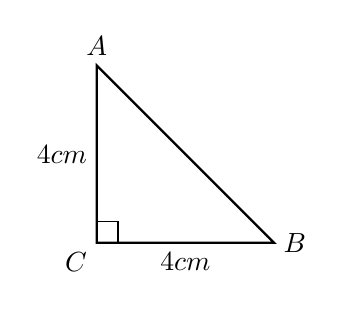
\begin{tikzpicture}[scale=0.9]
			\coordinate (A) at (0,2.5);
			\coordinate (C) at (0,0);
			\coordinate (B) at (2.5,0);
			
			\draw[thick] (A)--(C)--(B)--cycle;
			\draw (0,0) rectangle (0.3,0.3);
			
			\node [above] at (A) {$A$};
			\node [below left] at (C) {$C$};
			\node [right] at (B) {$B$};
			\node [left] at (0,1.25) {$4\text{ cm}$};
			\node [below] at (1.25,0) {$4\text{ cm}$};
		\end{tikzpicture}
		\caption{Isosceles right triangle $ABC$}
		\label{fig:EE26BTECH11223-10-4}
	\end{figure}
	
	\solution
	Triangle $ABC$ is an isosceles right-angled triangle at $C$. Since the hypotenuse $AB$ is the longest side, the two equal legs are $AC$ and $BC$:
	\begin{align}
		BC = AC = 4\text{ cm}
	\end{align}
	Applying the Pythagoras theorem \eqref{eq:CBSE10-2019-pythagoras} and \eqref{eq:CBSE10-2019-isosceles_right}:
	\begin{align}
		AB^2 &= AC^2 + BC^2 = 4^2 + 4^2 = 32 \\
		\implies AB &= \sqrt{32} = 4\sqrt{2}\text{ cm}
	\end{align}
	
	\item In \figref{fig:EE26BTECH11223-10-5}, $DE \parallel BC$. Find the length of side $AD$, given that $AE = 1.8\text{ cm}$, $BD = 7.2\text{ cm}$, and $CE = 5.4\text{ cm}$.
	\hfill (10~2019)
	\begin{figure}[H]
		\centering
		\begin{tikzpicture}[scale=0.95]
			\coordinate (A) at (2.4,4);
			\coordinate (C) at (0,0);
			\coordinate (B) at (4,1);
			\coordinate (D) at ($(A)!0.25!(B)$);
			\coordinate (E) at ($(A)!0.25!(C)$); 
			
			\draw[thick] (A)--(C)--(B)--cycle;
			\draw[thick] (D)--(E);
			
			\draw[->,thick] ($(D)!0.4!(E)$)--($(D)!0.55!(E)$);
			\draw[->,thick] ($(B)!0.4!(C)$)--($(B)!0.55!(C)$);
			
			\node [above] at (A) {$A$};
			\node [right] at (D) {$D$};
			\node [left] at (E) {$E$};
			\node [below left] at (B) {$B$};
			\node [below right] at (C) {$C$};
			
			\node [right] at ($(B)!0.55!(D)$) {$7.2\text{ cm}$};
			\node [left] at ($(A)!0.5!(E)$) {$1.8\text{ cm}$};
			\node [left] at ($(E)!0.5!(C)$) {$5.4\text{ cm}$};
		\end{tikzpicture}
		\caption{Triangle $ABC$ with $DE \parallel BC$}
		\label{fig:EE26BTECH11223-10-5}
	\end{figure}
	
	\solution
	In $\triangle ABC$, since $DE \parallel BC$, applying Thales' Theorem \eqref{eq:CBSE10-2019-thales}:
	\begin{align}
		\frac{AD}{BD} = \frac{AE}{CE}
	\end{align}
	Substituting the given lengths:
	\begin{align}
		\frac{AD}{7.2} = \frac{1.8}{5.4} = \frac{1}{3} \implies AD = \frac{7.2}{3} = 2.4\text{ cm}
	\end{align}
	
	\item Find the nature of roots of the quadratic equation $2x^2 - 4x + 3 = 0$.
	\hfill (10~2019)
	
	\solution
	Comparing with the standard quadratic form $ax^2 + bx + c = 0$:
	\begin{align}
		a = 2, \quad b = -4, \quad c = 3
	\end{align}
	From \eqref{eq:CBSE10-2019-discriminant}, the discriminant $D$ is:
	\begin{align}
		D = b^2 - 4ac = \brak{-4}^2 - 4\brak{2}\brak{3} = 16 - 24 = -8
	\end{align}
	Since $D < 0$, the quadratic equation has no real roots.
	The following code verifies the solution in \figref{fig:EE26BTECH11223-10-6}:
	\begin{lstlisting}[frame=single, basicstyle=\ttfamily\small]
		codes/10/q6.py
	\end{lstlisting}
	\begin{figure}[H]
		\centering
		\begin{tikzpicture}[scale=0.85]
			\draw[->] (-1,0) -- (3,0) node[right] {$x$};
			\draw[->] (0,-0.5) -- (0,5.5) node[above] {$y$};
			\draw[domain=-0.2:2.2, smooth, variable=\x, thick, blue] plot ({\x}, {2*\x*\x - 4*\x + 3});
			\fill (1,1) circle (2pt) node[right] {Vertex $(1,1)$};
			\node[above right, blue] at (1.4,3.8) {$y = 2x^2 - 4x + 3$};
		\end{tikzpicture}
		\caption{Plot of $y = 2x^2 - 4x + 3$ showing no real roots ($D < 0$)}
		\label{fig:EE26BTECH11223-10-6}
	\end{figure}
	
	\item If $\gcd\brak{336, 54} = 6$, find $\operatorname{lcm}\brak{336, 54}$.
	\hfill (10~2019)
	
	\solution
	Let $a = 336$ and $b = 54$. From \eqref{eq:CBSE10-2019-hcf_lcm}:
	\begin{align}
		\gcd\brak{a, b} \times \operatorname{lcm}\brak{a, b} = a \times b
	\end{align}
	Rearranging:
	\begin{align}
		\operatorname{lcm}\brak{336, 54} &= \frac{a \times b}{\gcd\brak{a, b}} \\
		&= \frac{336 \times 54}{6} = 336 \times 9 = 3024
	\end{align}
	
	\item Find the $21^{\text{st}}$ term of the A.P. $-4\frac{1}{2}, -3, -1\frac{1}{2}, \ldots$
	\hfill (10~2019)
	
	\solution
	The first term is $a = -\frac{9}{2}$. The common difference $d$ is:
	\begin{align}
		d = -3 - \brak{-\frac{9}{2}} = -3 + \frac{9}{2} = \frac{3}{2}
	\end{align}
	From \eqref{eq:CBSE10-2019-ap_nth_term}, the $n$-th term is:
	\begin{align}
		a_n = a + \brak{n - 1}d
	\end{align}
	Substituting $n = 21$:
	\begin{align}
		a_{21} &= -\frac{9}{2} + \brak{21 - 1}\brak{\frac{3}{2}} \\
		&= -\frac{9}{2} + 20\brak{\frac{3}{2}} = -\frac{9}{2} + 30 = \frac{51}{2} = 25\frac{1}{2}
	\end{align}
	
	\item For what value of $k$ will the system of equations $2x+3y=7$ and $(k+2)x-3(1-k)y=5k+1$ have infinitely many solutions?
	\hfill (10~2019)
	
	\solution
	Writing the system of linear equations in canonical matrix form $\mathbf{A}\vec{x} = \vec{b}$:
	\begin{align}
		\myvec{2 & 3 \\ k+2 & 3k-3}\myvec{x \\ y} = \myvec{7 \\ 5k+1}
	\end{align}
	The augmented matrix is
	\begin{align}
		\sbrak{\mathbf{A} \mid \vec{b}} = \myvec{2 & 3 & 7 \\ k+2 & 3k-3 & 5k+1}
	\end{align}
	Performing the elementary row operation $R_2 \to 2R_2 - (k+2)R_1$:
	\begin{align}
		\sbrak{\mathbf{A} \mid \vec{b}} \xrightarrow{R_2 \to 2R_2 - (k+2)R_1}
		\myvec{2 & 3 & 7 \\ 0 & 3k-12 & 3k-12}
	\end{align}
	From \eqref{eq:CBSE10-2019-rouche_capelli}, for the system to have infinitely many solutions:
	\begin{align}
		\rank\brak{\mathbf{A}} = \rank\brak{[\mathbf{A} \mid \vec{b}]} < 2
	\end{align}
	This requires the second row to be entirely zero:
	\begin{align}
		3k - 12 = 0 \implies k = 4
	\end{align}
	
	\item Find the mode of the following frequency distribution:
	\begin{center}
		\begin{tabular}{|c|c|c|c|c|c|c|}
			\hline
			Class Interval & 25--30 & 30--35 & 35--40 & 40--45 & 45--50 & 50--55\\
			\hline
			Frequency & 25 & 34 & 50 & 42 & 38 & 14\\
			\hline
		\end{tabular}
	\end{center}
	\hfill (10~2019)
	
	\solution
	The maximum frequency is $50$, corresponding to the modal class $35$--$40$.
	From the modal class:
	\begin{align}
		l = 35, \quad h = 5, \quad f_1 = 50, \quad f_0 = 34, \quad f_2 = 42
	\end{align}
	From \eqref{eq:CBSE10-2019-mode}, the mode is given by:
	\begin{align}
		\text{Mode} &= l + \brak{\frac{f_1 - f_0}{2f_1 - f_0 - f_2}} \times h \\
		&= 35 + \brak{\frac{50 - 34}{2\brak{50} - 34 - 42}} \times 5 \\
		&= 35 + \brak{\frac{16}{24}} \times 5 = 35 + \frac{10}{3} \approx 38.33
	\end{align}
	
	\item The larger of two supplementary angles exceeds the smaller by $18^\circ$. Find the angles.
	\hfill (10~2019)
	
	\solution
	Let the larger angle be $x$ and the smaller angle be $y$.
	Since the two angles are supplementary, their sum is $180^\circ$:
	\begin{align}
		x + y &= 180^\circ \label{eq:EE26BTECH11223-10-q11-eq1}
	\end{align}
	The larger angle exceeds the smaller by $18^\circ$:
	\begin{align}
		x - y &= 18^\circ \label{eq:EE26BTECH11223-10-q11-eq2}
	\end{align}
	Expressing the system of linear equations in canonical matrix form $\mathbf{M}\vec{x} = \vec{b}$:
	\begin{align}
		\myvec{1 & 1 \\ 1 & -1}\myvec{x \\ y} = \myvec{180^\circ \\ 18^\circ}
	\end{align}
	From \eqref{eq:CBSE10-2019-matrix_inverse}, evaluating the inverse matrix where $\mydet{\myvec{1 & 1 \\ 1 & -1}} = -1 - 1 = -2$:
	\begin{align}
		\myvec{x \\ y} &= \frac{1}{-2}\myvec{-1 & -1 \\ -1 & 1}\myvec{180^\circ \\ 18^\circ} \\
		&= \frac{1}{2}\myvec{1 & 1 \\ 1 & -1}\myvec{180^\circ \\ 18^\circ} = \frac{1}{2}\myvec{198^\circ \\ 162^\circ} = \myvec{99^\circ \\ 81^\circ}
	\end{align}
	Therefore, the two supplementary angles are $99^\circ$ and $81^\circ$.
	
	\item Sumit is $3$ times as old as his son. Five years later, he shall be two and a half times as old as his son. How old is Sumit at present?
	\hfill (10~2019)
	
	\solution
	Let the present age of the son be $x$ years and Sumit's present age be $y$ years.
	From the given conditions:
	\begin{align}
		y &= 3x \implies 3x - y = 0 \label{eq:EE26BTECH11223-10-q12-eq1}
	\end{align}
	Five years later, their ages will be $x + 5$ and $y + 5$ respectively:
	\begin{align}
		y + 5 &= \frac{5}{2}\brak{x + 5} \implies 2y + 10 = 5x + 25 \implies 5x - 2y = -15 \label{eq:EE26BTECH11223-10-q12-eq2}
	\end{align}
	Writing the system of equations in matrix form $\mathbf{A}\vec{x} = \vec{b}$:
	\begin{align}
		\myvec{3 & -1 \\ 5 & -2}\myvec{x \\ y} = \myvec{0 \\ -15}
	\end{align}
	From \eqref{eq:CBSE10-2019-matrix_inverse}, since $\mydet{\mathbf{A}} = 3\brak{-2} - \brak{-1}\brak{5} = -6 + 5 = -1$:
	\begin{align}
		\myvec{x \\ y} &= \frac{1}{-1}\myvec{-2 & 1 \\ -5 & 3}\myvec{0 \\ -15} = \myvec{2 & -1 \\ 5 & -3}\myvec{0 \\ -15} = \myvec{15 \\ 45}
	\end{align}
	Therefore, the present age of the son is $15\text{ years}$ and Sumit's present age is $45\text{ years}$.
	
	\item The probability of selecting a blue marble at random from a jar that contains only blue, black and green marbles is $\frac{1}{5}$. The probability of selecting a black marble at random from the same jar is $\frac{1}{4}$. If the jar contains $11$ green marbles, find the total number of marbles in the jar.
	\hfill (10~2019)
	
	\solution
	Let the total number of marbles in the jar be $n$.
	Let $B$, $K$, and $G$ denote the events of selecting a blue, black, and green marble, respectively.
	Since these events partition the sample space, from \eqref{eq:CBSE10-2019-prob_partition}:
	\begin{align}
		\pr{B} + \pr{K} + \pr{G} = 1
	\end{align}
	Substituting $\pr{B} = \frac{1}{5}$ and $\pr{K} = \frac{1}{4}$:
	\begin{align}
		\frac{1}{5} + \frac{1}{4} + \pr{G} = 1 \implies \frac{9}{20} + \pr{G} = 1 \implies \pr{G} = \frac{11}{20}
	\end{align}
	By the classical definition of probability:
	\begin{align}
		\pr{G} = \frac{n(G)}{n} \implies \frac{11}{20} = \frac{11}{n} \implies n = 20
	\end{align}
	Therefore, the total number of marbles in the jar is $20$.

	
	\item Find a relation between $x$ and $y$ if the points $A(x,y)$, $B(-4,6)$ and $C(-2,3)$ are collinear.
	\hfill (10~2019)
	
	\solution
	Let the position vectors of the given points be
	\begin{align}
		\vec{A} = \myvec{x \\ y}, \quad \vec{B} = \myvec{-4 \\ 6}, \quad \vec{C} = \myvec{-2 \\ 3}
	\end{align}
	Forming the displacement vectors relative to point $\vec{B}$:
	\begin{align}
		\vec{v}_1 &= \vec{A} - \vec{B} = \myvec{x - \brak{-4} \\ y - 6} = \myvec{x + 4 \\ y - 6} \\
		\vec{v}_2 &= \vec{C} - \vec{B} = \myvec{-2 - \brak{-4} \\ 3 - 6} = \myvec{2 \\ -3}
	\end{align}
	From \eqref{eq:CBSE10-2019-collinear}, points $\vec{A}, \vec{B}, \vec{C}$ are collinear if and only if the matrix formed by their displacement vectors has zero determinant:
	\begin{align}
		\mydet{\vec{v}_1 & \vec{v}_2} = 0 \implies \mydet{x + 4 & 2 \\ y - 6 & -3} = 0
	\end{align}
	Expanding the determinant:
	\begin{align}
		-3\brak{x + 4} - 2\brak{y - 6} = 0 \implies -3x - 12 - 2y + 12 = 0 \implies 3x + 2y = 0
	\end{align}
	The following code verifies the solution in \figref{fig:EE26BTECH11223-10-14}:
	\begin{lstlisting}[frame=single, basicstyle=\ttfamily\small]
		codes/10/q14.py
	\end{lstlisting}
	\begin{figure}[H]
		\centering
		\begin{tikzpicture}[scale=0.7]
			\draw[->] (-5.5,0) -- (3,0) node[right] {$x$};
			\draw[->] (0,-4) -- (0,7.5) node[above] {$y$};
			\draw[thick, blue, domain=-4.8:1.5] plot ({\x}, {-1.5*\x});
			\fill (-4,6) circle (2pt) node[above left] {$B(-4,6)$};
			\fill (-2,3) circle (2pt) node[below left] {$C(-2,3)$};
			\fill (0,0) circle (2pt) node[below right] {$A(0,0)$};
			\node[blue, right] at (1,-1.5) {$3x + 2y = 0$};
		\end{tikzpicture}
		\caption{Collinear points $A, B, C$ on the line $3x+2y=0$}
		\label{fig:EE26BTECH11223-10-14}
	\end{figure}
	
	\item Find the area of a triangle whose vertices are $(1,-1)$, $(-4,6)$ and $(-3,-5)$.
	\hfill (10~2019)
	
	\solution
	Let the position vectors of the vertices be
	\begin{align}
		\vec{A} = \myvec{1 \\ -1}, \quad \vec{B} = \myvec{-4 \\ 6}, \quad \vec{C} = \myvec{-3 \\ -5}
	\end{align}
	Forming the two displacement edge vectors from reference vertex $\vec{A}$:
	\begin{align}
		\vec{u} &= \vec{B} - \vec{A} = \myvec{-4 - 1 \\ 6 - \brak{-1}} = \myvec{-5 \\ 7} \\
		\vec{v} &= \vec{C} - \vec{A} = \myvec{-3 - 1 \\ -5 - \brak{-1}} = \myvec{-4 \\ -4}
	\end{align}
	From \eqref{eq:CBSE10-2019-triangle_area_det}, the area of $\triangle ABC$ is:
	\begin{align}
		\text{Area} &= \frac{1}{2}\abs{\mydet{\vec{u} & \vec{v}}} = \frac{1}{2}\abs{\mydet{-5 & -4 \\ 7 & -4}} \\
		&= \frac{1}{2}\abs{\brak{-5}\brak{-4} - \brak{-4}\brak{7}} = \frac{1}{2}\abs{20 + 28} = \frac{1}{2}\brak{48} = 24\text{ sq. units}
	\end{align}
	The following code verifies the solution in \figref{fig:EE26BTECH11223-10-15}:
	\begin{lstlisting}[frame=single, basicstyle=\ttfamily\small]
		codes/10/q15.py
	\end{lstlisting}
	\begin{figure}[H]
		\centering
		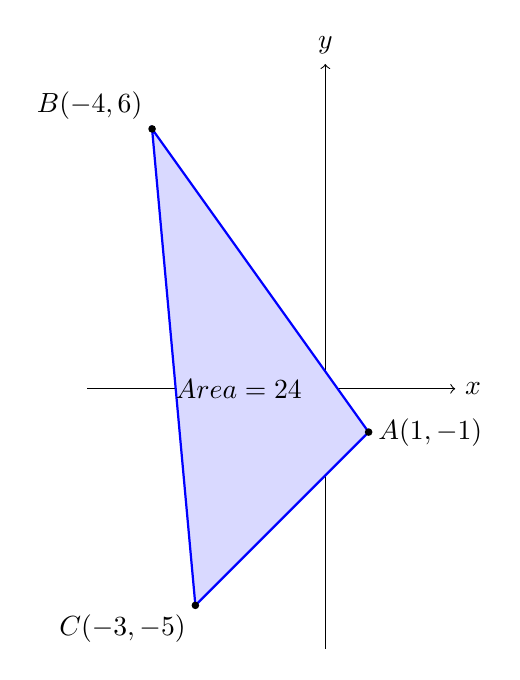
\begin{tikzpicture}[scale=0.55]
			\coordinate (A) at (1,-1);
			\coordinate (B) at (-4,6);
			\coordinate (C) at (-3,-5);
			\draw[->] (-5.5,0) -- (3,0) node[right] {$x$};
			\draw[->] (0,-6) -- (0,7.5) node[above] {$y$};
			\fill[blue!15] (A)--(B)--(C)--cycle;
			\draw[thick, blue] (A)--(B)--(C)--cycle;
			\fill (A) circle (2.5pt) node[right] {$A(1,-1)$};
			\fill (B) circle (2.5pt) node[above left] {$B(-4,6)$};
			\fill (C) circle (2.5pt) node[below left] {$C(-3,-5)$};
			\node at (-2,0) {$\text{Area} = 24$};
		\end{tikzpicture}
		\caption{Triangle $ABC$ with vertices $A(1,-1)$, $B(-4,6)$, and $C(-3,-5)$}
		\label{fig:EE26BTECH11223-10-15}
	\end{figure}
	
	\item Write the smallest number which is divisible by both $306$ and $657$.
	\hfill (10~2019)
	
	\solution
	The smallest positive integer divisible by both numbers is their least common multiple, $\operatorname{lcm}\brak{306, 657}$.
	Applying Euclid's division lemma:
	\begin{align}
		657 &= 306 \times 2 + 45 \\
		306 &= 45 \times 6 + 36 \\
		45 &= 36 \times 1 + 9 \\
		36 &= 9 \times 4 + 0
	\end{align}
	Since the remainder is $0$, the greatest common divisor is:
	\begin{align}
		\gcd\brak{306, 657} = 9
	\end{align}
	From \eqref{eq:CBSE10-2019-hcf_lcm}:
	\begin{align}
		\operatorname{lcm}\brak{306, 657} &= \frac{306 \times 657}{\gcd\brak{306, 657}} \\
		&= \frac{306 \times 657}{9} = 34 \times 657 = 22338
	\end{align}

	\item Point $A$ lies on the line segment $XY$ joining $X(6,-6)$ and $Y(-4,-1)$ in such a way that $\frac{XA}{XY}=\frac{2}{5}$. If point $A$ also lies on the line $3x+k(y+1)=0$, find the value of $k$.
	\hfill (10~2019)
	
	\solution
	Point $A$ lies on line segment $XY$ with position vectors $\vec{X} = \myvec{6 \\ -6}$ and $\vec{Y} = \myvec{-4 \\ -1}$.
	Given $\frac{XA}{XY} = \frac{2}{5}$, since $XY = XA + AY$:
	\begin{align}
		\frac{XA}{XA + AY} = \frac{2}{5} \implies 5 XA = 2 XA + 2 AY \implies 3 XA = 2 AY \implies \frac{XA}{AY} = \frac{2}{3}
	\end{align}
	Thus, point $\vec{A}$ divides the line segment joining $\vec{X}$ and $\vec{Y}$ internally in the ratio $m:n = 2:3$.
	From \eqref{eq:CBSE10-2019-section_formula}:
	\begin{align}
		\vec{A} &= \frac{m\vec{Y} + n\vec{X}}{m + n} = \frac{2\myvec{-4 \\ -1} + 3\myvec{6 \\ -6}}{2 + 3} \\
		&= \frac{1}{5}\brak{\myvec{-8 \\ -2} + \myvec{18 \\ -18}} = \frac{1}{5}\myvec{10 \\ -20} = \myvec{2 \\ -4}
	\end{align}
	Since point $\vec{A} = \myvec{2 \\ -4}$ lies on the line $3x + k\brak{y + 1} = 0$:
	\begin{align}
		3\brak{2} + k\brak{-4 + 1} = 0 \implies 6 - 3k = 0 \implies 3k = 6 \implies k = 2
	\end{align}
	The following code verifies the solution in \figref{fig:EE26BTECH11223-10-17}:
	\begin{lstlisting}[frame=single, basicstyle=\ttfamily\small]
		codes/10/q17.py
	\end{lstlisting}
	\begin{figure}[H]
		\centering
		\begin{tikzpicture}[scale=0.55]
			\coordinate (X) at (6,-6);
			\coordinate (Y) at (-4,-1);
			\coordinate (A) at (2,-4);
			\draw[->] (-5.5,0) -- (7.5,0) node[right] {$x$};
			\draw[->] (0,-7) -- (0,2) node[above] {$y$};
			\draw[thick, blue] (X) -- (Y);
			\fill (X) circle (2.5pt) node[right] {$X(6,-6)$};
			\fill (Y) circle (2.5pt) node[left] {$Y(-4,-1)$};
			\fill (A) circle (2.5pt) node[below left] {$A(2,-4)$};
			\draw[thick, red, domain=-1:5] plot ({\x}, {-3*\x/2 - 1});
			\node[red, above right] at (3.5,-6.25) {$3x + 2(y+1) = 0$};
		\end{tikzpicture}
		\caption{Point $A(2,-4)$ dividing $XY$ in ratio $2:3$}
		\label{fig:EE26BTECH11223-10-17}
	\end{figure}
	
	\item Solve for $x$:
	\begin{align}
		x^2 + 5x - \brak{a^2 + a - 6} = 0
	\end{align}
	\hfill (10~2019)
	
	\solution
	Comparing with the standard quadratic equation $Ax^2 + Bx + C = 0$:
	\begin{align}
		A = 1, \quad B = 5, \quad C = -\brak{a^2 + a - 6}
	\end{align}
	From \eqref{eq:CBSE10-2019-discriminant}, the discriminant $D$ is:
	\begin{align}
		D &= B^2 - 4AC = 5^2 - 4\brak{1}\sbrak{-\brak{a^2 + a - 6}} \\
		&= 25 + 4\brak{a^2 + a - 6} = 25 + 4a^2 + 4a - 24 \\
		&= 4a^2 + 4a + 1 = \brak{2a + 1}^2
	\end{align}
	Using the quadratic formula:
	\begin{align}
		x &= \frac{-B \pm \sqrt{D}}{2A} = \frac{-5 \pm \sqrt{\brak{2a + 1}^2}}{2\brak{1}} = \frac{-5 \pm \brak{2a + 1}}{2}
	\end{align}
	Taking the positive sign:
	\begin{align}
		x &= \frac{-5 + \brak{2a + 1}}{2} = \frac{2a - 4}{2} = a - 2
	\end{align}
	Taking the negative sign:
	\begin{align}
		x &= \frac{-5 - \brak{2a + 1}}{2} = \frac{-2a - 6}{2} = -\brak{a + 3}
	\end{align}
	Therefore, the roots are $x = a - 2$ or $x = -\brak{a + 3}$.

	\item Find $A$ and $B$ if $\sin(A+2B)=\frac{\sqrt{3}}{2}$ and $\cos(A+4B)=0$, where $A$ and $B$ are acute angles.
	\hfill (10~2019)
	
	\solution
	From \eqref{eq:CBSE10-2019-trig_values}, since $\sin\brak{60^\circ} = \frac{\sqrt{3}}{2}$ and angles are acute:
	\begin{align}
		A + 2B &= 60^\circ \label{eq:EE26BTECH11223-10-q19-eq1}
	\end{align}
	Since $\cos\brak{90^\circ} = 0$:
	\begin{align}
		A + 4B &= 90^\circ \label{eq:EE26BTECH11223-10-q19-eq2}
	\end{align}
	Expressing the system of linear equations in matrix form $\mathbf{M}\vec{x} = \vec{b}$:
	\begin{align}
		\myvec{1 & 2 \\ 1 & 4}\myvec{A \\ B} = \myvec{60^\circ \\ 90^\circ}
	\end{align}
	From \eqref{eq:CBSE10-2019-matrix_inverse}, evaluating the determinant and inverse of $\mathbf{M}$:
	\begin{align}
		\mydet{\mathbf{M}} = \mydet{1 & 2 \\ 1 & 4} = 1\brak{4} - 2\brak{1} = 2
	\end{align}
	\begin{align}
		\mathbf{M}^{-1} = \frac{1}{2}\myvec{4 & -2 \\ -1 & 1}
	\end{align}
	Solving for the angles:
	\begin{align}
		\myvec{A \\ B} &= \frac{1}{2}\myvec{4 & -2 \\ -1 & 1}\myvec{60^\circ \\ 90^\circ} \\
		&= \frac{1}{2}\myvec{4\brak{60^\circ} - 2\brak{90^\circ} \\ -1\brak{60^\circ} + 1\brak{90^\circ}} = \frac{1}{2}\myvec{240^\circ - 180^\circ \\ -60^\circ + 90^\circ} = \frac{1}{2}\myvec{60^\circ \\ 30^\circ} = \myvec{30^\circ \\ 15^\circ}
	\end{align}
	Therefore, $A = 30^\circ$ and $B = 15^\circ$.

	\item Prove that $2+5\sqrt{3}$ is an irrational number, given that $\sqrt{3}$ is an irrational number.
	\hfill (10~2019)
	
	\solution
	Assume to the contrary that $2 + 5\sqrt{3}$ is a rational number.
	Then it can be written in the form $\frac{a}{b}$, where $a, b \in \mathbb{Z}$, $b \ne 0$, and $\gcd\brak{a, b} = 1$:
	\begin{align}
		2 + 5\sqrt{3} &= \frac{a}{b}
	\end{align}
	Rearranging the terms:
	\begin{align}
		5\sqrt{3} &= \frac{a}{b} - 2 = \frac{a - 2b}{b} \\
		\implies \sqrt{3} &= \frac{a - 2b}{5b} \label{eq:EE26BTECH11223-10-q20-contra}
	\end{align}
	Since $a$ and $b$ are integers, $a - 2b$ and $5b$ are also integers with $5b \ne 0$. Thus, the right-hand side represents a rational number:
	\begin{align}
		\frac{a - 2b}{5b} \in \mathbb{Q} \implies \sqrt{3} \in \mathbb{Q}
	\end{align}
	This contradicts the given fact that $\sqrt{3}$ is an irrational number.
	Hence, our assumption was false, and $2 + 5\sqrt{3}$ is an irrational number.

	
	
	\item Using Euclid's Algorithm, find the HCF of $2048$ and $960$.
	\hfill (10~2019)
	
	\solution
	From \eqref{eq:CBSE10-2019-euclid_shear}, the reduction of an integer state vector under elementary unimodular shear matrices preserves the greatest common divisor:
	\begin{align}
		\vec{v}_0 = \myvec{2048 \\ 960}
	\end{align}
	Applying the first shear transformation $\mathbf{E}_1 = \myvec{1 & -2 \\ 0 & 1}$:
	\begin{align}
		\vec{v}_1 = \mathbf{E}_1 \vec{v}_0 = \myvec{1 & -2 \\ 0 & 1}\myvec{2048 \\ 960} = \myvec{2048 - 2\brak{960} \\ 960} = \myvec{128 \\ 960}
	\end{align}
	Applying the second shear transformation $\mathbf{E}_2 = \myvec{1 & 0 \\ -7 & 1}$:
	\begin{align}
		\vec{v}_2 = \mathbf{E}_2 \vec{v}_1 = \myvec{1 & 0 \\ -7 & 1}\myvec{128 \\ 960} = \myvec{128 \\ 960 - 7\brak{128}} = \myvec{128 \\ 64}
	\end{align}
	Applying the third shear transformation $\mathbf{E}_3 = \myvec{1 & -2 \\ 0 & 1}$:
	\begin{align}
		\vec{v}_3 = \mathbf{E}_3 \vec{v}_2 = \myvec{1 & -2 \\ 0 & 1}\myvec{128 \\ 64} = \myvec{128 - 2\brak{64} \\ 64} = \myvec{0 \\ 64}
	\end{align}
	The non-zero invariant entry of the reduced state vector yields:
	\begin{align}
		\gcd\brak{2048, 960} = 64
	\end{align}
	The following code verifies the solution:

	\item Two right triangles $ABC$ and $DBC$ are drawn on the same hypotenuse $BC$ and on the same side of $BC$. If $AC$ and $BD$ intersect at $P$, prove that $AP\times PC=BP\times DP$.
	\hfill (10~2019)
	\begin{figure}[H]
		\centering
		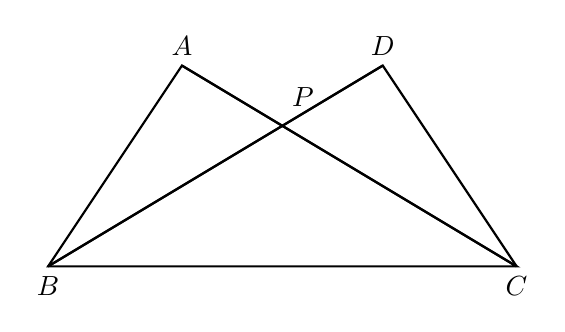
\begin{tikzpicture}[scale=0.85]
			\coordinate (B) at (0,0);
			\coordinate (C) at (7,0);
			\coordinate (A) at (2,3);
			\coordinate (D) at (5,3);
			\coordinate (P) at (3.5,2.25);
			
			\draw[thick] (B)--(A)--(C)--cycle;
			\draw[thick] (B)--(D)--(C);
			\draw[thick] (A)--(C);
			\draw[thick] (B)--(D);
			
			\node[above] at (A) {$A$};
			\node[above] at (D) {$D$};
			\node[below] at (B) {$B$};
			\node[below] at (C) {$C$};
			\node[above right] at (P) {$P$};
		\end{tikzpicture}
		\caption{Right triangles $ABC$ and $DBC$ on the common hypotenuse $BC$}
		\label{fig:EE26BTECH11223-10-22}
	\end{figure}
	
	\solution
	In right triangles $ABC$ and $DBC$, both are right-angled with hypotenuse $BC$:
	\begin{align}
		\angle BAC = 90^\circ, \quad \angle BDC = 90^\circ
	\end{align}
	Since the hypotenuse $BC$ subtends equal angles of $90^\circ$ at vertices $A$ and $D$ on the same side of $BC$, points $A, B, C, D$ are concyclic and lie on a circle with diameter $BC$.
	For the chord $AD$, angles in the same segment of the circle are equal:
	\begin{align}
		\angle PBA = \angle PCD
	\end{align}
	In $\triangle PAB$ and $\triangle PDC$:
	\begin{align}
		\angle APB &= \angle DPC \quad \brak{\text{vertically opposite angles}} \\
		\angle PBA &= \angle PCD \quad \brak{\text{angles in the same segment}}
	\end{align}
	By the AA similarity criterion, $\triangle PAB \sim \triangle PDC$.
	From \eqref{eq:CBSE10-2019-intersecting_chords}, the corresponding sides are proportional:
	\begin{align}
		\frac{AP}{DP} = \frac{BP}{PC} \implies AP \times PC = BP \times DP
	\end{align}
	The following code verifies the geometric property:

	
	\item Diagonals of a trapezium $PQRS$ intersect each other at the point $O$, $PQ\parallel RS$ and $PQ=3RS$. Find the ratio of the areas of triangles $POQ$ and $ROS$.
	\hfill (10~2019)
	\begin{figure}[H]
		\centering
		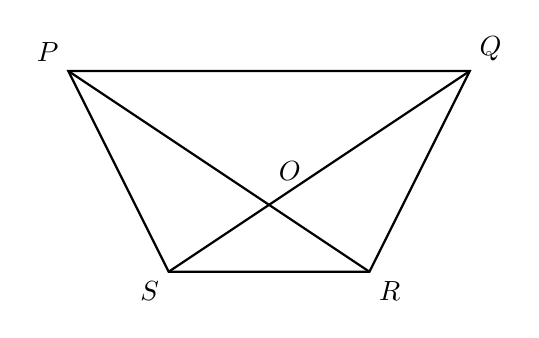
\begin{tikzpicture}[scale=0.85]
			\coordinate (P) at (0,3);
			\coordinate (Q) at (6,3);
			\coordinate (R) at (4.5,0);
			\coordinate (S) at (1.5,0);
			\coordinate (O) at (3,1.5);
			
			\draw[thick] (P)--(Q)--(R)--(S)--cycle;
			\draw[thick] (P)--(R);
			\draw[thick] (Q)--(S);
			
			\node[above left] at (P) {$P$};
			\node[above right] at (Q) {$Q$};
			\node[below right] at (R) {$R$};
			\node[below left] at (S) {$S$};
			\node[right] at (O) {$O$};
		\end{tikzpicture}
		\caption{Trapezium $PQRS$ with diagonals intersecting at $O$}
		\label{fig:EE26BTECH11223-10-23}
	\end{figure}
	
	\solution
	In trapezium $PQRS$, given $PQ \parallel RS$. In $\triangle POQ$ and $\triangle ROS$:
	\begin{align}
		\angle POQ &= \angle ROS \quad \brak{\text{vertically opposite angles}} \\
		\angle OPQ &= \angle ORS \quad \brak{\text{alternate interior angles, since } PQ \parallel RS} \\
		\angle OQP &= \angle OSR \quad \brak{\text{alternate interior angles, since } PQ \parallel RS}
	\end{align}
	Therefore, by the AAA similarity criterion, $\triangle POQ \sim \triangle ROS$.
	From \eqref{eq:CBSE10-2019-similar_triangle_area}:
	\begin{align}
		\frac{\text{ar}\brak{\triangle POQ}}{\text{ar}\brak{\triangle ROS}} = \brak{\frac{PQ}{RS}}^2
	\end{align}
	Given that $PQ = 3RS$:
	\begin{align}
		\frac{\text{ar}\brak{\triangle POQ}}{\text{ar}\brak{\triangle ROS}} = \brak{\frac{3RS}{RS}}^2 = 3^2 = \frac{9}{1}
	\end{align}
	Thus, the ratio of the areas of $\triangle POQ$ and $\triangle ROS$ is $9:1$.
	The following code verifies the area ratio:

	
	\item In \figref{fig:EE26BTECH11223-10-24}, $PQ$ and $RS$ are two parallel tangents to a circle with centre $O$ and another tangent $AB$ with point of contact $C$ intersects $PQ$ at $A$ and $RS$ at $B$. Prove that $\angle AOB=90^\circ$.
	\hfill (10~2019)
	\begin{figure}[H]
		\centering
		\begin{tikzpicture}[>=Stealth, line cap=round, line join=round, thick]
			\def\r{2.0}
			\def\alphaAng{55}
			
			\coordinate (O) at (0, 0);
			\coordinate (D) at (0, \r);
			\coordinate (E) at (0, -\r);
			
			\pgfmathsetmacro{\xA}{\r * tan(\alphaAng)}
			\pgfmathsetmacro{\xB}{\r * tan(90 - \alphaAng)}
			\pgfmathsetmacro{\angC}{90 - 2*\alphaAng}
			
			\coordinate (A) at (\xA, \r);
			\coordinate (B) at (\xB, -\r);
			\coordinate (C) at (\angC:\r);
			
			\draw (O) circle (\r);
			\draw [<->] (-2.5, \r) -- (4.2, \r);
			\draw [<->] (-2.5, -\r) -- (4.2, -\r);
			
			\draw (A) -- (B);
			\draw (O) -- (A);
			\draw (O) -- (B);
			
			\fill (O) circle (1.8pt) node[left=1pt] {$O$};
			\fill (D) circle (1.8pt) node[above=2pt] {$D$};
			\fill (E) circle (1.8pt) node[below=2pt] {$E$};
			\fill (A) circle (1.8pt) node[above=2pt] {$A$};
			\fill (B) circle (1.8pt) node[below=2pt] {$B$};
			\fill (C) circle (1.8pt) node[right=2pt] {$C$};
			
			\node[above] at (-2.0, \r) {$P$};
			\node[above] at (3.6, \r) {$Q$};
			\node[below] at (-2.0, -\r) {$R$};
			\node[below] at (3.6, -\r) {$S$};
		\end{tikzpicture}
		\caption{Parallel tangents $PQ, RS$ and transversal tangent $AB$}
		\label{fig:EE26BTECH11223-10-24}
	\end{figure}
	
	\solution
	Let the centre $O$ be the coordinate origin $\myvec{0 \\ 0}$.
	The parallel tangents $PQ$ and $RS$ correspond to the horizontal hyperplanes $y = r$ and $y = -r$.
	From \eqref{eq:CBSE10-2019-circle_tangent}, let the point of contact $C$ on the circle $\norm{\vec{x}} = r$ be parameterized by:
	\begin{align}
		\vec{r}_C = \myvec{r\cos\theta \\ r\sin\theta}, \quad \theta \in \brak{-\frac{\pi}{2}, \frac{\pi}{2}}
	\end{align}
	The tangent line at $C$ with normal $\hat{n} = \myvec{\cos\theta \\ \sin\theta}$ has equation:
	\begin{align}
		x\cos\theta + y\sin\theta = r
	\end{align}
	Intersecting with $y = r$ (line $PQ$) and $y = -r$ (line $RS$):
	\begin{align}
		\vec{r}_A = \myvec{r\frac{1 - \sin\theta}{\cos\theta} \\ r}, \quad \vec{r}_B = \myvec{r\frac{1 + \sin\theta}{\cos\theta} \\ -r}
	\end{align}
	From \eqref{eq:CBSE10-2019-orthogonality}, evaluating the scalar product $\vec{r}_A^\top \vec{r}_B$:
	\begin{align}
		\vec{r}_A^\top \vec{r}_B &= r^2 \brak{\frac{1 - \sin\theta}{\cos\theta}}\brak{\frac{1 + \sin\theta}{\cos\theta}} + r\brak{-r} \\
		&= r^2 \brak{\frac{1 - \sin^2\theta}{\cos^2\theta}} - r^2 = r^2\brak{1} - r^2 = 0
	\end{align}
	Since $\vec{r}_A^\top \vec{r}_B = 0$, $\vec{OA} \perp \vec{OB}$, which proves that $\angle AOB = 90^\circ$.
	The following code verifies the orthogonality:

	
	\item In \figref{fig:EE26BTECH11223-10-25}, a square $OABC$ is inscribed in a quadrant $OPBQ$. If $OA=15\text{ cm}$, find the area of the shaded region. (Use $\pi=3.14$.)
	\hfill (10~2019)
	\begin{figure}[H]
		\centering
		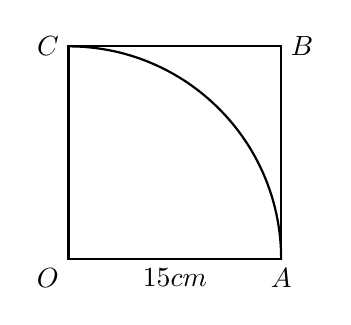
\begin{tikzpicture}[scale=0.18]
			\coordinate (O) at (0,0);
			\coordinate (A) at (15,0);
			\coordinate (B) at (15,15);
			\coordinate (C) at (0,15);
			
			\fill[gray!30] (O)--(15,0) arc (0:90:15)--cycle;
			\fill[white] (O)--(A)--(B)--(C)--cycle;
			
			\draw[thick] (O)--(15,0);
			\draw[thick] (O)--(0,15);
			\draw[thick] (15,0) arc (0:90:15);
			\draw[thick] (O)--(A)--(B)--(C)--cycle;
			
			\node[below left] at (O) {$O$};
			\node[below] at (A) {$A$};
			\node[right] at (B) {$B$};
			\node[left] at (C) {$C$};
			\node[below] at (7.5,0) {$15\text{ cm}$};
		\end{tikzpicture}
		\caption{Square $OABC$ inscribed in circular quadrant $OPBQ$}
		\label{fig:EE26BTECH11223-10-25}
	\end{figure}
	
	\solution
	From \eqref{eq:CBSE10-2019-square_geometry}, the side length of square $OABC$ is $s = OA = 15\text{ cm}$.
	Applying Pythagoras theorem \eqref{eq:CBSE10-2019-pythagoras} in right-angled $\triangle OAB$, diagonal $OB$ forms the radius $r$ of quadrant $OPBQ$:
	\begin{align}
		r^2 = OB^2 = OA^2 + AB^2 = 15^2 + 15^2 = 450 \implies r = 15\sqrt{2}\text{ cm}
	\end{align}
	From \eqref{eq:CBSE10-2019-quadrant_area}, the area of quadrant $OPBQ$ is:
	\begin{align}
		\text{Area of quadrant} &= \frac{1}{4}\pi r^2 = \frac{1}{4}\brak{3.14}\brak{450} = \frac{1413}{4} = 353.25\text{ cm}^2
	\end{align}
	The area of square $OABC$ is:
	\begin{align}
		\text{Area of square} &= s^2 = 15^2 = 225\text{ cm}^2
	\end{align}
	Therefore, the area of the shaded region is:
	\begin{align}
		\text{Area of shaded region} &= \text{Area of quadrant} - \text{Area of square} \\
		&= 353.25 - 225 = 128.25\text{ cm}^2
	\end{align}
	The following code verifies the solution:

	\item In \figref{fig:EE26BTECH11223-10-26}, $ABCD$ is a square with side $2\sqrt{2}\text{ cm}$ and inscribed in a circle. Find the area of the shaded region. (Use $\pi=3.14$.)
	\hfill (10~2019)
	\begin{figure}[H]
		\centering
		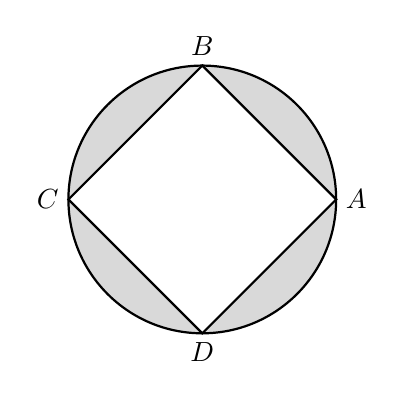
\begin{tikzpicture}[scale=0.85]
			\coordinate (O) at (0,0);
			\coordinate (A) at (2,0);
			\coordinate (B) at (0,2);
			\coordinate (C) at (-2,0);
			\coordinate (D) at (0,-2);
			
			\fill[gray!30] (O) circle (2);
			\fill[white] (A)--(B)--(C)--(D)--cycle;
			
			\draw[thick] (O) circle (2);
			\draw[thick] (A)--(B)--(C)--(D)--cycle;
			
			\node[right] at (A) {$A$};
			\node[above] at (B) {$B$};
			\node[left] at (C) {$C$};
			\node[below] at (D) {$D$};
		\end{tikzpicture}
		\caption{Square $ABCD$ inscribed in circumscribed circle}
		\label{fig:EE26BTECH11223-10-26}
	\end{figure}
	
	\solution
	Let the side of the inscribed square $ABCD$ be $s = 2\sqrt{2}\text{ cm}$.
	Since each interior angle of the square is $90^\circ$, diagonal $AC$ is the diameter of the circle.
	From \eqref{eq:CBSE10-2019-pythagoras}:
	\begin{align}
		AC^2 = AB^2 + BC^2 = \brak{2\sqrt{2}}^2 + \brak{2\sqrt{2}}^2 = 8 + 8 = 16 \implies AC = 4\text{ cm}
	\end{align}
	Thus, the radius of the circle is:
	\begin{align}
		r = \frac{AC}{2} = \frac{4}{2} = 2\text{ cm}
	\end{align}
	From \eqref{eq:CBSE10-2019-circumscribed_circle}, the area of the circle is:
	\begin{align}
		\text{Area of circle} &= \pi r^2 = 3.14 \times 2^2 = 12.56\text{ cm}^2
	\end{align}
	The area of the inscribed square is:
	\begin{align}
		\text{Area of square} &= s^2 = \brak{2\sqrt{2}}^2 = 8\text{ cm}^2
	\end{align}
	The area of the shaded region is:
	\begin{align}
		\text{Area of shaded region} &= \text{Area of circle} - \text{Area of square} \\
		&= 12.56 - 8 = 4.56\text{ cm}^2
	\end{align}
	The following code verifies the solution:

	\item A solid is in the form of a cylinder with hemispherical ends. The total height of the solid is $20\text{ cm}$ and the diameter of the cylinder is $7\text{ cm}$. Find the total volume of the solid. (Use $\pi=\frac{22}{7}$.)
	\hfill (10~2019)
	\begin{figure}[H]
		\centering
		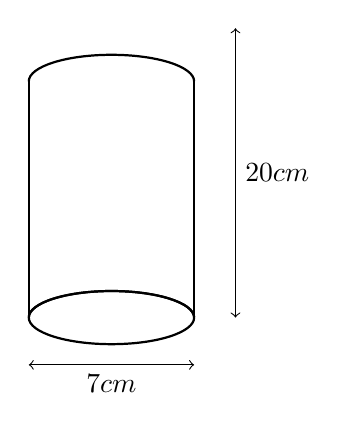
\begin{tikzpicture}[scale=0.75]
			\draw[thick] (0,0) arc (180:360:1.4 and 0.45);
			\draw[thick] (0,0) arc (180:0:1.4 and 0.45);
			\draw[thick] (0,0)--(0,4);
			\draw[thick] (2.8,0)--(2.8,4);
			\draw[thick] (0,4) arc (180:0:1.4 and 0.45);
			\draw[thick] (0,0) arc (180:0:1.4 and 0.45);
			
			\draw[<->] (3.5,0)--(3.5,4.9);
			\node[right] at (3.5,2.45) {$20\text{ cm}$};
			\draw[<->] (0,-0.8)--(2.8,-0.8);
			\node[below] at (1.4,-0.8) {$7\text{ cm}$};
		\end{tikzpicture}
		\caption{Cylinder with hemispherical ends}
		\label{fig:EE26BTECH11223-10-27}
	\end{figure}
	
	\solution
	The diameter is $d = 7\text{ cm}$, giving radius $r = \frac{7}{2}\text{ cm}$.
	Total height of the solid is $H = 20\text{ cm}$.
	The height of the cylindrical body $h$ is:
	\begin{align}
		h = H - 2r = 20 - 2\brak{\frac{7}{2}} = 20 - 7 = 13\text{ cm}
	\end{align}
	From \eqref{eq:CBSE10-2019-vol_cylinder}, the volume of the cylindrical portion is:
	\begin{align}
		V_{\text{cyl}} &= \pi r^2 h = \frac{22}{7} \times \brak{\frac{7}{2}}^2 \times 13 = \frac{22}{7} \times \frac{49}{4} \times 13 = \frac{1001}{2} = 500.5\text{ cm}^3
	\end{align}
	From \eqref{eq:CBSE10-2019-vol_sphere}, the two hemispherical ends combine to form a sphere:
	\begin{align}
		V_{\text{ends}} &= 2 \times \brak{\frac{2}{3}\pi r^3} = \frac{4}{3}\pi r^3 = \frac{4}{3} \times \frac{22}{7} \times \brak{\frac{7}{2}}^3 = \frac{539}{3} \approx 179.67\text{ cm}^3
	\end{align}
	The total volume of the solid is:
	\begin{align}
		V = V_{\text{cyl}} + V_{\text{ends}} = \frac{1001}{2} + \frac{539}{3} = \frac{3003 + 1078}{6} = \frac{4081}{6} \approx 680.17\text{ cm}^3
	\end{align}
	The following code verifies the computed volume:
	\begin{lstlisting}[frame=single, basicstyle=\ttfamily\small]
		codes/10/q27.py
	\end{lstlisting}
	
	\item The marks obtained by $100$ students in an examination are given below:
	\begin{center}
		\begin{tabular}{|l|c|c|c|c|c|c|c|}
			\hline
			Marks & 30--35 & 35--40 & 40--45 & 45--50 & 50--55 & 55--60 & 60--65\\
			\hline
			Number of Students & 14 & 16 & 28 & 23 & 18 & 8 & 3\\
			\hline
		\end{tabular}
	\end{center}
	Find the mean marks of the students.
	\hfill (10~2019)
	
	\solution
	Constructing the computation table with class marks $x_i = \frac{l_i + u_i}{2}$:
	\begin{center}
		\begin{tabular}{|c|c|c|c|}
			\hline
			Class Interval & Class Mark ($x_i$) & Frequency ($f_i$) & $f_i x_i$ \\
			\hline
			30--35 & 32.5 & 14 & 455.0 \\
			35--40 & 37.5 & 16 & 600.0 \\
			40--45 & 42.5 & 28 & 1190.0 \\
			45--50 & 47.5 & 23 & 1092.5 \\
			50--55 & 52.5 & 18 & 945.0 \\
			55--60 & 57.5 & 8  & 460.0 \\
			60--65 & 62.5 & 3  & 187.5 \\
			\hline
			\textbf{Total} & & $\sum f_i = 110$ & $\sum f_i x_i = 4930.0$ \\
			\hline
		\end{tabular}
	\end{center}
	From \eqref{eq:CBSE10-2019-mean}, the arithmetic mean is:
	\begin{align}
		\bar{x} = \frac{\sum_{i=1}^k f_i x_i}{\sum_{i=1}^k f_i} = \frac{4930}{110} = \frac{493}{11} \approx 44.82
	\end{align}
	The following code verifies the solution in \figref{fig:EE26BTECH11223-10-28}:
	\begin{lstlisting}[frame=single, basicstyle=\ttfamily\small]
		codes/10/q28.py
	\end{lstlisting}

	
	\item For what value of $k$ is the polynomial $f(x)=3x^4-9x^3+x^2+15x+k$ completely divisible by $3x^2-5$?
	\hfill (10~2019)
	
	\solution
	From \eqref{eq:CBSE10-2019-poly_mod}, work in the quotient ring $\mathbb{R}[x] / \langle 3x^2 - 5 \rangle$, where the divisor induces the reduction relation:
	\begin{align}
		3x^2 - 5 \equiv 0 \implies x^2 \equiv \frac{5}{3}
	\end{align}
	Higher powers of the state variable $x$ reduce algebraically:
	\begin{align}
		x^3 &= x \cdot x^2 \equiv \frac{5}{3}x \\
		x^4 &= \brak{x^2}^2 \equiv \brak{\frac{5}{3}}^2 = \frac{25}{9}
	\end{align}
	Projecting $f(x)$ modulo $3x^2 - 5$:
	\begin{align}
		f(x) &\equiv 3\brak{\frac{25}{9}} - 9\brak{\frac{5}{3}x} + \brak{\frac{5}{3}} + 15x + k \\
		&\equiv \frac{25}{3} - 15x + \frac{5}{3} + 15x + k \\
		&\equiv \frac{30}{3} + k \equiv 10 + k \pmod{3x^2 - 5}
	\end{align}
	For $f(x)$ to be completely divisible, the remainder residue must be zero:
	\begin{align}
		10 + k = 0 \implies k = -10
	\end{align}
	The following code verifies the polynomial division:
	\begin{lstlisting}[frame=single, basicstyle=\ttfamily\small]
		codes/10/q29.py
	\end{lstlisting}
	
	\item Find the zeroes of the quadratic polynomial $7y^2-\frac{11}{3}y-\frac{2}{3}$ and verify the relationship between the zeroes and the coefficients.
	\hfill (10~2019)
	
	\solution
	To find the zeroes, set $p(y) = 7y^2 - \frac{11}{3}y - \frac{2}{3} = 0$.
	Multiplying by $3$:
	\begin{align}
		21y^2 - 11y - 2 = 0
	\end{align}
	Factoring by splitting the middle term:
	\begin{align}
		21y^2 - 14y + 3y - 2 &= 0 \\
		7y\brak{3y - 2} + 1\brak{3y - 2} &= 0 \\
		\brak{3y - 2}\brak{7y + 1} &= 0
	\end{align}
	Equating each factor to zero:
	\begin{align}
		3y - 2 = 0 \implies y = \frac{2}{3}, \qquad 7y + 1 = 0 \implies y = -\frac{1}{7}
	\end{align}
	Thus, the zeroes are $\alpha = \frac{2}{3}$ and $\beta = -\frac{1}{7}$.
	
	Comparing $p(y)$ with the standard quadratic polynomial $ay^2 + by + c$:
	\begin{align}
		a = 7, \quad b = -\frac{11}{3}, \quad c = -\frac{2}{3}
	\end{align}
	Verifying Vieta's relations \eqref{eq:CBSE10-2019-vieta_sum} and \eqref{eq:CBSE10-2019-vieta_prod}:
	\begin{align}
		\alpha + \beta &= \frac{2}{3} + \brak{-\frac{1}{7}} = \frac{14 - 3}{21} = \frac{11}{21} = -\frac{-11/3}{7} = -\frac{b}{a} \\
		\alpha \beta &= \brak{\frac{2}{3}}\brak{-\frac{1}{7}} = -\frac{2}{21} = \frac{-2/3}{7} = \frac{c}{a}
	\end{align}
	Hence, the relationship between zeroes and coefficients is verified.

	
	\item Prove that the ratio of the areas of two similar triangles is equal to the ratio of the squares on their corresponding sides.
	\hfill (10~2019)
	
	\solution
	Let $\triangle ABC \sim \triangle PQR$. Draw altitudes $AM \perp BC$ and $PN \perp QR$.
	The ratio of their areas is:
	\begin{align}
		\frac{\text{ar}\brak{\triangle ABC}}{\text{ar}\brak{\triangle PQR}} = \frac{\frac{1}{2} BC \times AM}{\frac{1}{2} QR \times PN} = \brak{\frac{BC}{QR}}\brak{\frac{AM}{PN}}
	\end{align}
	In $\triangle ABM$ and $\triangle PQN$, $\angle B = \angle Q$ (as $\triangle ABC \sim \triangle PQR$) and $\angle AMB = \angle PNQ = 90^\circ$. By AA similarity:
	\begin{align}
		\triangle ABM \sim \triangle PQN \implies \frac{AM}{PN} = \frac{AB}{PQ}
	\end{align}
	Since $\triangle ABC \sim \triangle PQR$, the corresponding sides are proportional:
	\begin{align}
		\frac{AB}{PQ} = \frac{BC}{QR} = \frac{CA}{RP}
	\end{align}
	Substituting $\frac{AM}{PN} = \frac{BC}{QR}$ yields \eqref{eq:CBSE10-2019-similar_triangle_area}:
	\begin{align}
		\frac{\text{ar}\brak{\triangle ABC}}{\text{ar}\brak{\triangle PQR}} = \brak{\frac{AB}{PQ}}^2 = \brak{\frac{BC}{QR}}^2 = \brak{\frac{CA}{FD}}^2
	\end{align}
	
	\item Two poles of equal heights are standing opposite to each other on either side of the road which is $80\text{ m}$ wide. From a point $P$ between them on the road, the angle of elevation of the top of a pole is $60^\circ$ and the angle of depression from the top of the other pole to point $P$ is $30^\circ$. Find the heights of the poles and the distance of the point $P$ from the poles.
	\hfill (10~2019)
	\begin{figure}[H]
		\centering
		\begin{tikzpicture}[scale=0.8,>=Stealth]
			\draw[thick] (0,0)--(10,0);
			\draw[thick] (0,0)--(0,4);
			\draw[thick] (10,0)--(10,4);
			
			\coordinate (P) at (3,0);
			\fill (P) circle (2pt);
			\node[below] at (P) {$P$};
			
			\coordinate (T1) at (0,4);
			\coordinate (T2) at (10,4);
			
			\draw[dashed] (P)--(T1);
			\draw[dashed] (P)--(T2);
			\draw[dotted] (10,4)--(3,4);
			
			\node[left] at (T1) {Top};
			\node[right] at (T2) {Top};
			\node[below] at (1.5,0) {$x$};
			\node[below] at (6.5,0) {$80-x$};
			\node[above] at (5,4) {Horizontal line};
			
			\draw (P) ++(0.7,0) arc (0:53:0.7);
			\node at (4.0,0.45) {$60^\circ$};
			
			\draw (10,4) ++(-0.8,0) arc (180:225:0.8);
			\node at (8.9,3.45) {$30^\circ$};
			
			\node[below] at (5,-0.8) {Road width $=80\text{ m}$};
		\end{tikzpicture}
		\caption{Poles and point of observation on road}
		\label{fig:EE26BTECH11223-10-32}
	\end{figure}
	
	\solution
	Let the height of both poles be $h$ and the distance of $P$ from the first pole be $x$.
	From the angles of elevation and depression:
	\begin{align}
		\tan\brak{60^\circ} = \frac{h}{x} \implies h = \sqrt{3}x \label{eq:EE26BTECH11223-10-pole1} \\
		\tan\brak{30^\circ} = \frac{h}{80 - x} \implies h = \frac{80 - x}{\sqrt{3}} \label{eq:EE26BTECH11223-10-pole2}
	\end{align}
	Equating \eqref{eq:EE26BTECH11223-10-pole1} and \eqref{eq:EE26BTECH11223-10-pole2}:
	\begin{align}
		\sqrt{3}x = \frac{80 - x}{\sqrt{3}} \implies 3x = 80 - x \implies 4x = 80 \implies x = 20\text{ m}
	\end{align}
	The height of each pole is:
	\begin{align}
		h = 20\sqrt{3}\text{ m}
	\end{align}
	The distance from the second pole is $80 - 20 = 60\text{ m}$.

	
	\item The total cost of a certain length of a piece of cloth is Rs.~200. If the piece was $5\text{ m}$ longer and each metre of cloth costs Rs.~2 less, the cost of the piece would have remained unchanged. How long is the piece and what is its original rate per metre?
	\hfill (10~2019)
	
	\solution
	Let the original length of cloth be $x$ metres.
	The original rate per metre is $\frac{200}{x}$.
	With the new conditions:
	\begin{align}
		\brak{x + 5}\brak{\frac{200}{x} - 2} = 200
	\end{align}
	Expanding:
	\begin{align}
		200 - 2x + \frac{1000}{x} - 10 &= 200 \\
		-2x - 10 + \frac{1000}{x} &= 0 \\
		x^2 + 5x - 500 &= 0
	\end{align}
	Factoring:
	\begin{align}
		\brak{x + 25}\brak{x - 20} = 0 \implies x = 20\text{ m} \quad (\text{since } x > 0)
	\end{align}
	The original rate is:
	\begin{align}
		\text{Rate} = \frac{200}{20} = 10\text{ Rs./m}
	\end{align}

	
	\item Which term of the Arithmetic Progression $-7,\,-12,\,-17,\,-22,\,\ldots $ will be $-82$? Is $-100$ any term of the A.P.? Give reason for your answer.
	\hfill (10~2019)
	
	\solution
	Here, $a = -7$ and $d = -12 - \brak{-7} = -5$.
	From \eqref{eq:CBSE10-2019-ap_nth_term}:
	\begin{align}
		a_n = a + \brak{n - 1}d
	\end{align}
	Setting $a_n = -82$:
	\begin{align}
		-82 = -7 + \brak{n - 1}\brak{-5} \implies -75 = -5\brak{n - 1} \implies n = 16
	\end{align}
	Thus, the $16^{\text{th}}$ term is $-82$.
	Now testing $-100$:
	\begin{align}
		-100 = -7 + \brak{m - 1}\brak{-5} \implies -93 = -5\brak{m - 1} \implies m = 1 + \frac{93}{5} = 19.6
	\end{align}
	Since $m \notin \mathbb{Z}^^+$, $-100$ is not a term of the A.P.
	The following code verifies the solution:

	\item Change the following data into a ``less than type'' distribution and draw its ogive:
	\begin{center}
		\begin{tabular}{|c|c|c|c|c|c|c|c|}
			\hline
			Class Interval & 30--40 & 40--50 & 50--60 & 60--70 & 70--80 & 80--90 & 90--100\\
			\hline
			Frequency & 7 & 5 & 8 & 10 & 6 & 6 & 8\\
			\hline
		\end{tabular}
	\end{center}
	\hfill (10~2019)
	
	\solution
	The cumulative frequency table for the ``less than type'' distribution using the upper class limits:
	\begin{center}
		\begin{tabular}{|c|c|c|}
			\hline
			Marks (Upper Limit) & Frequency ($f$) & Cumulative Frequency ($cf$) \\
			\hline
			Less than 40 & 7 & 7 \\
			Less than 50 & 5 & 12 \\
			Less than 60 & 8 & 20 \\
			Less than 70 & 10 & 30 \\
			Less than 80 & 6 & 36 \\
			Less than 90 & 6 & 42 \\
			Less than 100 & 8 & 50 \\
			\hline
			\textbf{Total} & $N = 50$ & \\
			\hline
		\end{tabular}
	\end{center}
	Plotting points $\brak{30, 0}, \brak{40, 7}, \brak{50, 12}, \brak{60, 20}, \brak{70, 30}, \brak{80, 36}, \brak{90, 42}, \brak{100, 50}$ on the Cartesian plane yields the ogive curve.
	Here, total observations $N = 50$:
	\begin{align}
		\frac{N}{2} = \frac{50}{2} = 25
	\end{align}
	Locating $25$ on the $y$-axis and projecting onto the ogive curve, the corresponding value on the $x$-axis gives the median:
	\begin{align}
		\text{Median} = 65
	\end{align}

	\item Draw two concentric circles of radii $2\text{ cm}$ and $5\text{ cm}$. Take a point $P$ on the outer circle and construct a pair of tangents $PA$ and $PB$ to the smaller circle. Measure $PA$.
	\hfill (10~2019)
	
	\solution
	Let the common centre be $\vec{O} = \myvec{0 \\ 0}$. Point $\vec{P}$ lies on the outer circle such that $\norm{\vec{P}} = 5\text{ cm}$.
	Since $PA$ is tangent to the inner circle of radius $r = 2\text{ cm}$ at point $A$, radius $\vec{OA}$ is orthogonal to tangent $\vec{PA}$ ($\vec{OA} \perp \vec{PA}$).
	Applying Pythagoras theorem \eqref{eq:CBSE10-2019-pythagoras} in right-angled $\triangle OAP$:
	\begin{align}
		PA^2 = OP^2 - OA^2 = 5^2 - 2^2 = 25 - 4 = 21 \implies PA = \sqrt{21} \approx 4.58\text{ cm}
	\end{align}
	
	The following code generates the geometric construction:
	\begin{lstlisting}[frame=single, basicstyle=\ttfamily\small]
		codes/10/q36.py
	\end{lstlisting}
	


	\item A solid iron pole consists of a cylinder of height $220\text{ cm}$ and base diameter $24\text{ cm}$, which is surmounted by another cylinder of height $60\text{ cm}$ and radius $8\text{ cm}$. Find the mass of the pole, given that $1\text{ cm}^3$ of iron has approximately $8\text{ gm}$ mass. (Use $\pi=3.14$.)
	\hfill (10~2019)
	
	\solution
	The iron pole consists of two coaxial right circular cylinders stacked vertically.
	
	\text{Lower (Larger) Cylinder:}
	\begin{align}
		h_1 = 220\text{ cm}, \quad r_1 = \frac{24}{2} = 12\text{ cm}
	\end{align}
	From \eqref{eq:CBSE10-2019-vol_cylinder}, the volume of the lower cylinder is:
	\begin{align}
		V_1 = \pi r_1^2 h_1 = 3.14 \times 12^2 \times 220 = 3.14 \times 144 \times 220 = 99475.2\text{ cm}^3
	\end{align}
	
	\text{Upper (Smaller) Cylinder:}
	\begin{align}
		h_2 = 60\text{ cm}, \quad r_2 = 8\text{ cm}
	\end{align}
	The volume of the upper cylinder is:
	\begin{align}
		V_2 = \pi r_2^2 h_2 = 3.14 \times 8^2 \times 60 = 3.14 \text{64} \times 60 = 12057.6\text{ cm}^3
	\end{align}
	
	\text{Total Volume:}
	\begin{align}
		V = V_1 + V_2 = 99475.2 + 12057.6 = 111532.8\text{ cm}^3
	\end{align}
	
	\text{Total Mass:}
	From \eqref{eq:CBSE10-2019-mass_density}, with density $\rho = 8\text{ gm/cm}^3$:
	\begin{align}
		\text{Mass} = V \times \rho = 111532.8 \times 8 = 892262.4\text{ gm} = 892.26\text{ kg}
	\end{align}5
	
	
\end{enumerate}